\subsection{Dinámica: Movimiento Circular}
\label{sec:mcu}

El movimiento circular es un movimiento acelerado. Al ser la trayectoria una circunferencia, es necesario que exista una aceleración para cambiar la dirección y el sentido de la velocidad en cada punto. La posición de una partícula en una circunferencia podemos determinarla de forma general en función del ángulo barrido. Entonces podemos definir las siguientes cantidades:

\begin{tcolorbox}[remember, title=Posición angular (\(\theta\))]
  La posición angular indica el ángulo barrido respecto a un eje fijo.
  \[
  \theta(t) = \theta_0 + \omega_0 t + \frac{1}{2} \alpha t^2
  \]
  donde:
  \begin{itemize}
    \item \(\theta_0\) es la posición angular inicial,
    \item \(\omega_0\) es la velocidad angular inicial,
    \item \(\alpha\) es la aceleración angular.
  \end{itemize}
\end{tcolorbox}

\begin{tcolorbox}[remember, title=Velocidad angular (\(\omega\))]
La velocidad angular mide el cambio de la posición angular respecto al tiempo.
\[
\omega(t) = \omega_0 + \alpha t
\]
Y también:
\[
\omega^2 = \omega_0^2 + 2\alpha(\theta - \theta_0)
\]
Esta última es útil si desea eliminar el tiempo de la ecuación. Si se pide relacionar el tipo de movimiento con la frecuencia:
\[
  \omega = 2 \pi f
\]
\end{tcolorbox}

\begin{tcolorbox}[remember, title=Aceleración angular (\(\alpha\))]  
Es la razón de cambio de la velocidad angular:
\[
\alpha = \frac{d\omega}{dt}
\]
\end{tcolorbox}
Como vemos las cantidades definidas para un movimiento circular no dependen del radio de la circunferencia que realiza la partícula estudiada. 
\begin{figure}[ht]
  \centering
  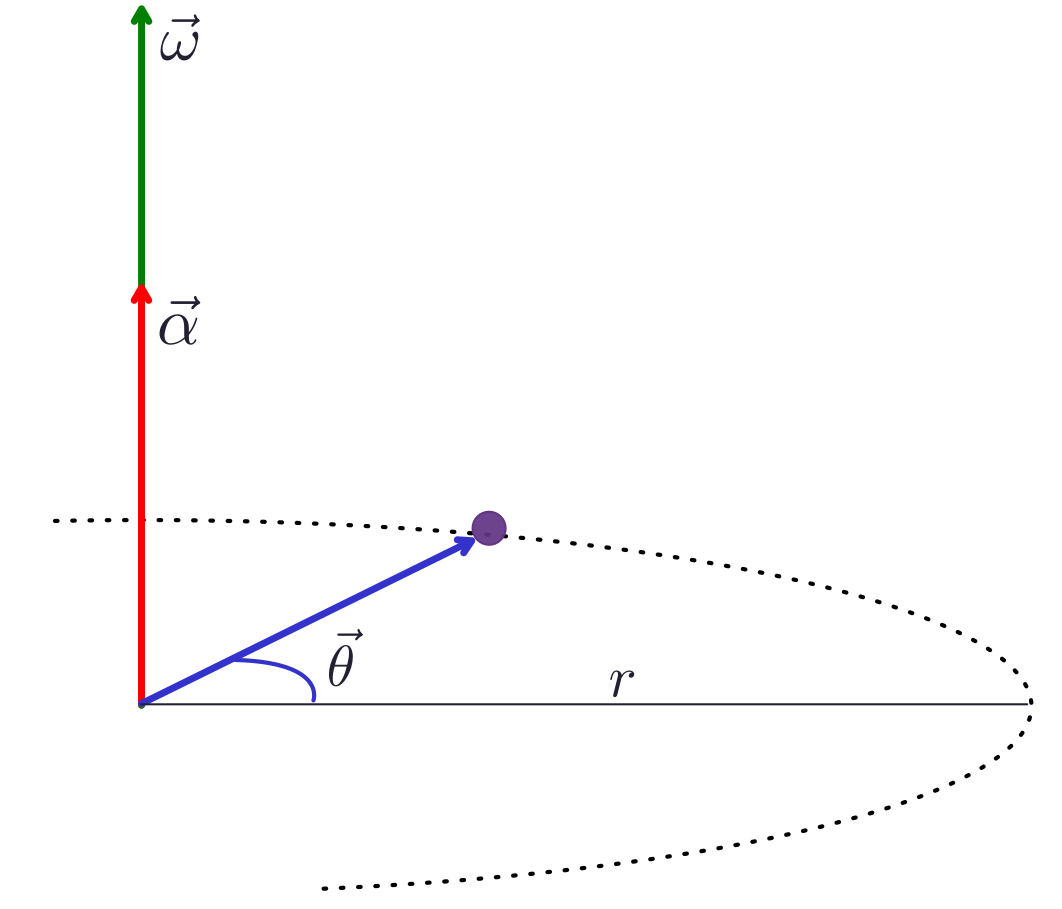
\includegraphics[width=0.37\textwidth]{mcu.png}
  \caption{Elementos del movimiento circular}
\end{figure}
Para poder relacionar estas cantidades con el radio y con distancias métricas podemos usar la definición de arco. Entonces un desplazamiento \(S\) será:
\[
S = \left\lvert \Delta \theta \right\rvert \cdot \text{Radio}
\]
A partir de esta cantidad podemos definir las siguientes cantidades:
\begin{tcolorbox}[remember, title=Velocidad tangencial (\(v_t\))]  
La velocidad lineal de un punto situado a una distancia \( r \) del eje de rotación es:
\[
v_t = r \, \omega
\]
La dirección de \( v_t \) es siempre tangente a la trayectoria circular.
\end{tcolorbox}

\begin{tcolorbox}[remember, title=Aceleración centrípeta (\(a_c\))]
La aceleración centrípeta está directamente relacionada con la velocidad tangencial en el movimiento circular. Su relación es:
\[
a_c = \frac{v_t^2}{r}
\]
Esta aceleración siempre está presente y se encarga de cambiar la dirección del vector velocidad en cada punto.
\end{tcolorbox}

\begin{tcolorbox}[remember, title=Aceleración tangencial (\(a_t\))]
La aceleración tangencial está asociada al cambio en el módulo de la velocidad tangencial y por lo tanto, a la aceleración angular:
\[
a_t = r \, \alpha
\]
\end{tcolorbox}

\begin{tcolorbox}[remember, title=Fuerza centrípeta (\(F_c\))]
La fuerza necesaria para mantener un cuerpo en movimiento circular uniforme (o no uniforme) está dirigida hacia el centro de la trayectoria:
\[
F_c = m \frac{v_t^2}{r} = m r \omega^2
\]
donde \( m \) es la masa del objeto.
\end{tcolorbox}

\begin{figure}[ht]
  \centering
  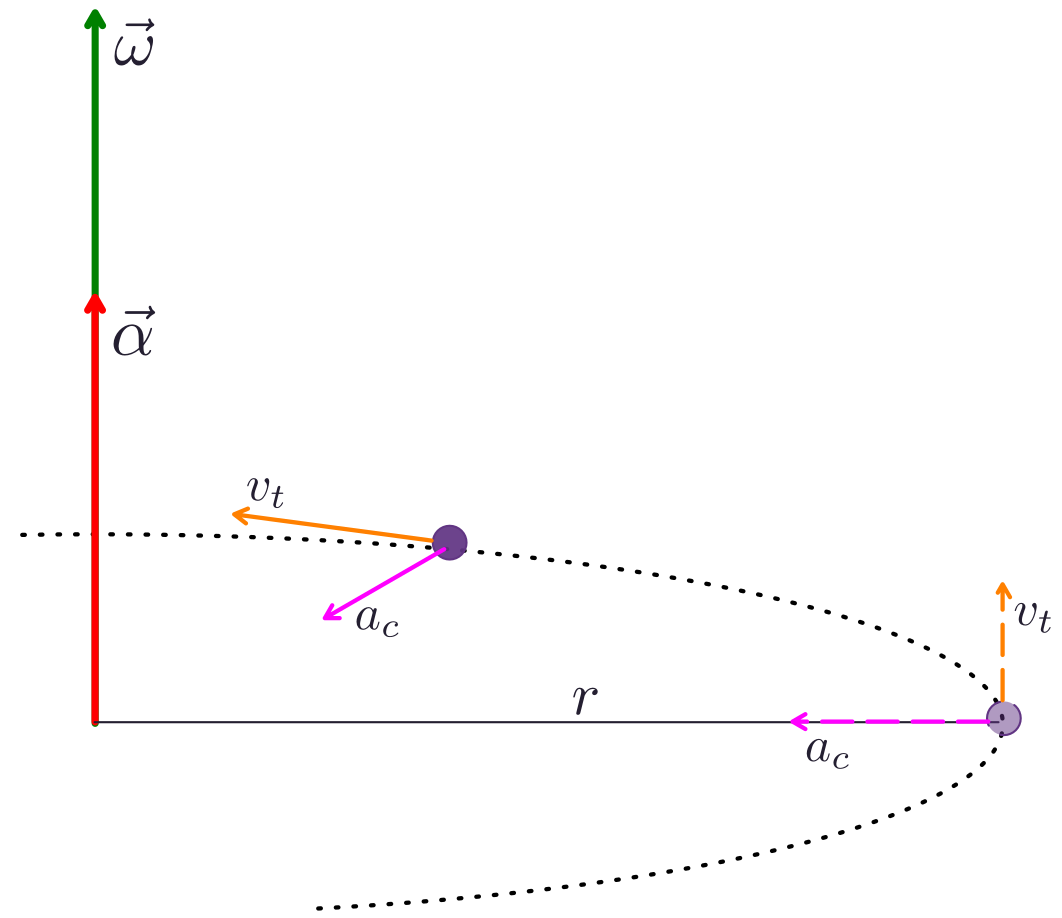
\includegraphics[width=0.37\textwidth]{mcu_r.png}
  \caption{Velocidad tangencial y aceleración centrípeta}
\end{figure}